\documentclass{beamer}
\usepackage{sdp}

\title{Потоци}

\titlegraphic{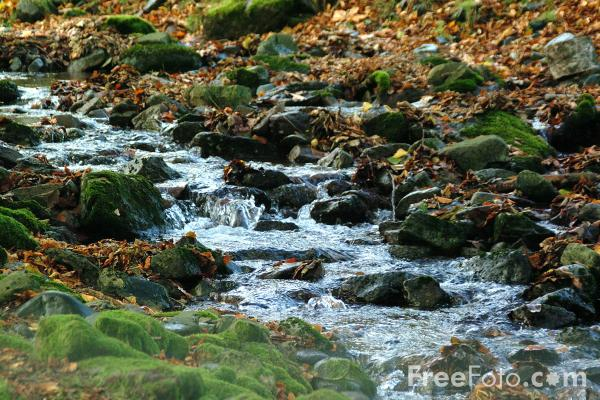
\includegraphics[width=0.5\textwidth]{images/stream.jpg}}

\begin{document}

\begin{frame}
  \titlepage
\end{frame}

\begin{frame}
  \frametitle{Взаимодействие на две програми}

  Програма А пресмята поредица от данни
  \begin{itemize}
  \item простите числа
  \item кадри от видео клип
  \item списък от постове във Facebook/Twitter
  \end{itemize}
  \vspace{1em}
  
  Програма Б обработва поредица от данни
  \begin{itemize}
  \item търси числа-близнаци
  \item прави снимки на ``интересни'' моменти от
    клипа
  \item събира всички постове с линк към YouTube
  \end{itemize}
  \vspace{2em}
  
  \alert{Как да организираме работата на двете програми?}
\end{frame}

\begin{frame}
  \frametitle{Абстракцията поток}

  \begin{center}
    производител
    $\longrightarrow$ 
\includegraphics[width=0.4\textwidth,valign=c]{images/abstract_stream.pdf}
    $\longrightarrow$ консуматор
  \end{center}
\end{frame}

\begin{frame}
  \frametitle{Обектно-ориентиран подход}

  \tt{cin >{}> number >{}> char >{}> string;}
  \vspace{2em}

  \tt{file <{}< student <{}< list <{}< tree;}
  \vspace{2em}
  
  \tt{while (stream1 >{}> x) stream2 <{}< f(x);}
\end{frame}

\begin{frame}
  \frametitle{Конвейерна обработка}

  \begin{itemize}
  \item събирането на няколко потока в един голям поток
  \item ефективна паралелна обработка
  \item саморегулиращ се механизъм
  \item Пример: Unix pipes
  \item \tt{ls | grep new | wc -l}
  \item Файловете като производители или консуматори на потоци
  \end{itemize}
\end{frame}

\begin{frame}
  \frametitle{Поточен буфер}

  \begin{itemize}
  \item Какво представлява буферът?
  \item Кога е нужен буфер?
  \item Кога буферът вреди?
  \end{itemize}
  \vspace{2em}

  \begin{tabular}{|c|c|c|c|c|c|c|c|c|c|c|c|c|c|}
    \rowcolor{blue!60!green!40}
    \hline
    H&e&l&l&o&,& &w&o&r&l&d&!&\tt{\textbackslash n}\\
    \hline
  \end{tabular}
\end{frame}

\begin{frame}
  \frametitle{Стандартни потоци и пренасочване}

  \begin{itemize}
  \item Стандартен изходен поток \tt{cout} (\tt{stdout})
    \begin{itemize}
    \item Пренасочване на изхода:
    \item \tt{ls  > filelist.txt}
    \end{itemize}
  \item Стандартен входен поток \tt{cin} (\tt{stdin})
    \begin{itemize}
    \item Пренасочване на вход и на изход:
    \item \tt{grep password < email.txt > password.txt}
    \end{itemize}
  \item Стандартен поток за грешки \tt{cerr} (\tt{stderr})
    \begin{itemize}
    \item Пренасочване на изход за грешки:
    \item \tt{mv *.dat /data 2> errors.txt}
    \end{itemize}
  \item Стандартен поток за дневник \tt{clog} (отново \tt{stderr})    
  \end{itemize}
\end{frame}

\begin{frame}
  \frametitle{Поточна йерархия в C++}

  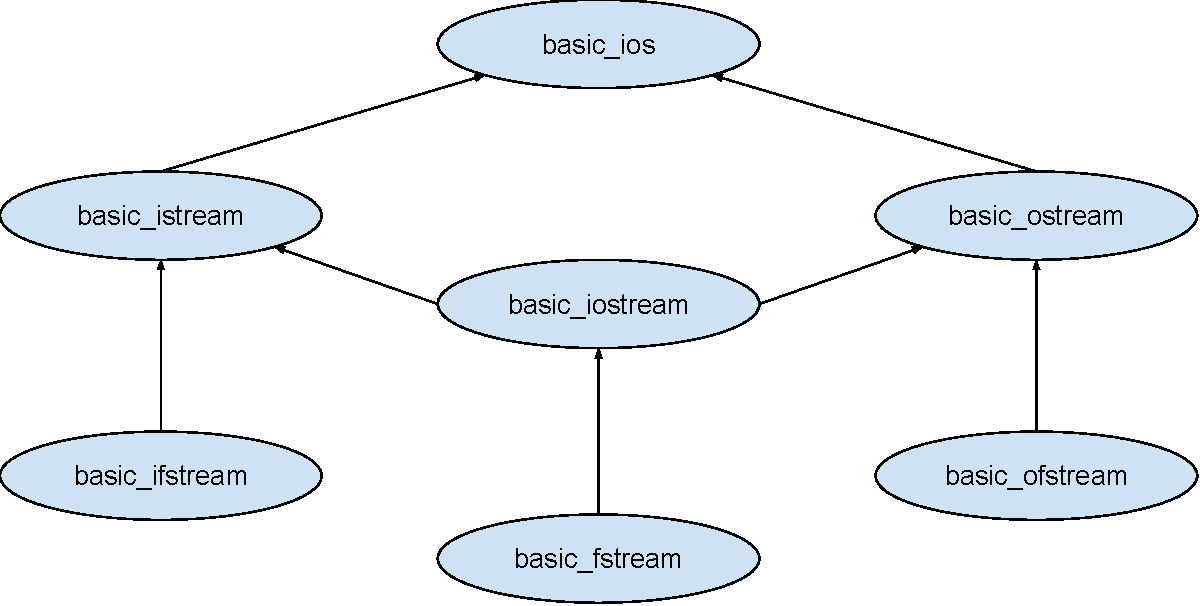
\includegraphics[width=\textwidth]{images/stream_hierarchy.pdf}
\end{frame}

\begin{frame}
  \frametitle{Форматиран и неформатиран вход/изход}

  \begin{itemize}
  \item Текстова и двоична информация
  \item ASCII (\tt{char})
  \item Служебни символи
  \item Кодиращи таблици
  \item Unicode (\tt{wchar\_t})
  \item UTF-8
  \end{itemize}
\end{frame}

\begin{frame}[fragile]
  \frametitle{Изход на поток}

  Неформатиран изход:
  \vspace{1em}

  \verb#ostream& put(char);#

  \verb#ostream& write(const char*, streamsize);#

  \vspace{3em}

  Форматиран изход:
  \vspace{1em}
  
  \verb#ostream& operator<<(ostream&, T);#
\end{frame}

\begin{frame}[fragile]
  \frametitle{Вход от поток}

  Неформатиран вход:
  \vspace{1em}

  \verb#istream& get(char&);#\\
  \verb#istream& get(char*,streamsize,char);#\\
  \verb#istream& getline(char*,streamsize,char);#\\
  \verb#streamsize gcount() const;#\\
  \verb#istream& read(char*, streamsize);#
  \vspace{2em}

  Форматиран вход:
  \vspace{1em}

  \verb#istream& operator>>(istream&, T&);#  

  \vspace{2em}

  Допълнителни функции:

  \verb#int peek();#\\
  \verb#istream& putback(char);#
\end{frame}

\begin{frame}[fragile]
  \frametitle{Низови потоци}
  
  \verb@#include <sstream>@
  \vspace{1em}

  Входен поток от низ: \tt{istringstream}
  \vspace{1em}

  Пример:
\begin{verbatim}
char s[] = "1 2 3";
istringstream iss(s);
int a, b, c;
iss >> a >> b >> c;
\end{verbatim}
  \vspace{1em}

  Изходен поток към низ: \tt{ostringstream}
  \vspace{1em}
  
  Пример:
\begin{verbatim}
ostringstream oss;
oss << 1.2 << ' ' << 3.4;
cout << oss.str();
\end{verbatim}
\end{frame}

\begin{frame}[fragile]
  \frametitle{Състояние на поток}
  
  Флагове за състояние:\vspace{1em}
  \begin{tabular}{|c||c|c|c|c|}
    \hline
    \multirow{2}{*}{\tt{iostate}}&\tt{goodbit}&\tt{eofbit}&\tt{failbit}&\tt{badbit}\\
    \cline{2-5}
    &0&1&2&4\\
    \hline
  \end{tabular}
  \vspace{1em}

  Селектори:

  \verb#bool good() const;#
  \verb#bool eof() const;#\\
  \verb#bool fail() const;#
  \verb#bool bad() const;#\\
  \verb#iostate rdstate() const;#
  \vspace{1em}

  Мутатор:

  \verb#void clear(iostate = 0);#
  \vspace{1em}
  
  Примери:

  \verb#if (cin.rdstate() & (eofbit | badbit)) ...#\\
  \verb#cin.clear(failbit);#\\
  \verb#if(cin)...#\hskip 10ex\verb#if(!cin)...#

\end{frame}

\begin{frame}[fragile]
  \frametitle{Потокови манипулатори}

  \verb@#include<iomanip>@\\
  \verb#stream << data1 << manipulator << data2;#

  \begin{itemize}
  \item Манипулатори за изход: \tt{endl}, \tt{ends}, \tt{flush}
  \item Манипулатори за бройна система: \tt{hex}, \tt{oct}, \tt{dec}
  \item Манипулатори за поле: \tt{setw}, \tt{setfill}, \tt{left}, \tt{right}, \tt{internal}
  \item Манипулатори за дробни числа: \tt{fixed}, \tt{scientific}, \tt{setprecision}
  \item Манипулатори за формат: \tt{setiosflags}, \tt{setbase}
  \item \ldots и много други
  \end{itemize}
\end{frame}

\end{document}
